Voici une présentation de l'interface et ses fonctionnalités.

\subsection{Interface}
Voici comment se présente notre interface : 
\begin{figure}[!h]
    \centering
    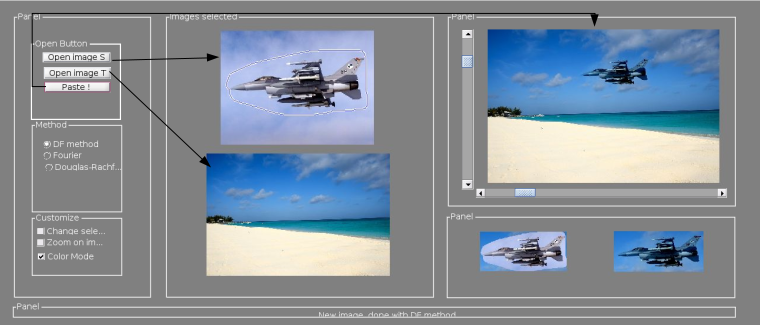
\includegraphics[scale = 0.5]{Images/interface.png}
    \caption{Interface 1.0}
\end{figure}{}
\subsubsection{Ouverture d'images}
Vous pouvez ouvrir n'importe quelle image en cliquant sur les boutons situés en haut à gauche de l'interface. En cliquant sur eux, une boite de dialogue vous proposera de choisir une image présente sur votre ordinateur. Une fois sélectionnée cette image sera affichée sur l'interface et vous pourrez travailler dessus. Image S correspond à l'image Source, c'est l'image que vous souhaitez coller. Et l'image T représente l'image Target, l'image d'arrière plan.\newline
\subsubsection{Sélection}
Une fois vos deux images ouvertes, il vous faut sélectionner la partie de l'image S (8) que vous souhaitez coller dans l'image T. Pour cela cliquez une première fois sur l'image S : celle du haut puis cliquez une seconde fois pour dessiner sur l'image, la partie que vous souhaitez extraire. 
\newline
Pour la seconde image, faites de même (9), cliquez une première fois sur l'image puis cliquez une seconde fois pour choisir l'endroit où vous souhaitez coller la partie sélectionnée plus tôt.  Voici ce que vous devriez obtenir. 
\subsubsection{Choix des méthodes}
Vous pouvez sélectionner la méthode avec laquelle vous voulez coller l'image S dans l'image T. Vous avez pour l'instant deux méthodes : 
\begin{itemize}
    \item Avec les différences finies (4)
    \item Avec Fourier (5)
\end{itemize}{}

\subsubsection{Différences finies}
Une fois la méthode DF choisie, il vous suffit de cliquer sur le bouton "Paste!"(3)  pour afficher le résultat.
\subsubsection{Options}
Nous avons ajoutés des options comme l'option de zoom (6) qui permet de zoomer sur une image pour voir de plus près le collage de l'image. 
\paragraph{ Amélioration avec change selection}
Ainsi nous avons ajouté, l'option Change sélection qui re-dimensionne automatique la sélection afin de résoudre ce pb. 
\paragraph{Mode couleur}
En sélectionnant le mode couleur, (8) vous pourrez travailler sur des images en couleur. 

\subsubsection{Sliders}
Vous pouvez bouger les sliders présents à droite afin de déplacer la zone collée dans l'image de fond. La solution au problème est alors automatiquement recalculée en fonction de l'endroit où l'objet à collé. 

\subsection{Organisation du code}
Nous avons organisé le code sous forme de classes. Le projet contient 2 classes principales, la classe, Fourier et la classe DFinies

%%%%%%%%%%%%%%%%%%%%%%%%%%%%%%%%%%%%%%%%%%%%%%%%%%%

\begin{figure}
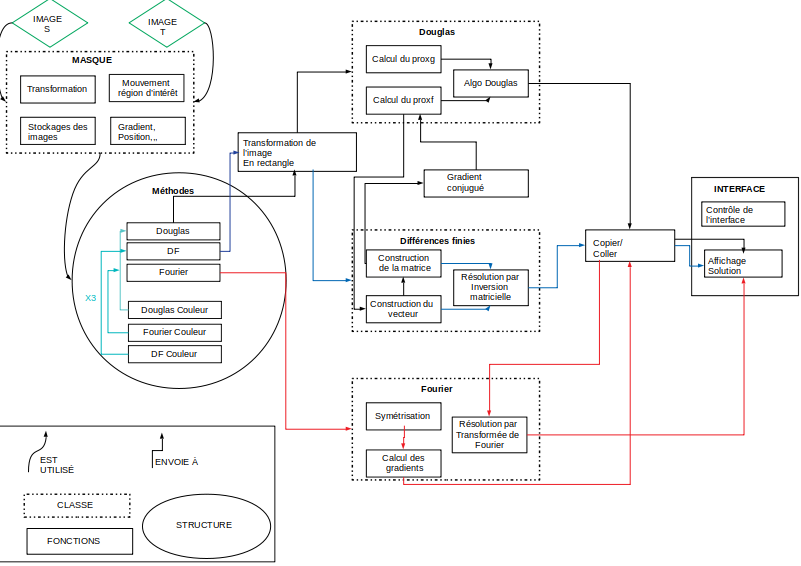
\includegraphics[scale=0.65]{Images/code/schema.png}
\end{figure}